\section{Análisis de objetivos y metodología}
En este apartado se detallarán los aspectos previos a la resolución del proyecto: los objetivos, las herramientas a utilizar para resolverlo, así como la instalación de una cámara que deberá hacerse para obtener imágenes de juego.

\subsection{Objetivos del proyecto}
En este trabajo se tratará de, usando imágenes de una cámara en vista cenital, desarrollar un sistema capaz de detectar y seguir (mediante \textit{tracking}) de manera robusta tanto los jugadores como balón de un partido de volleyball. Las imágenes de la cámara serán como las que pueden verse en la figura \ref{fig:campo}.

\begin{figure}
    \centering
    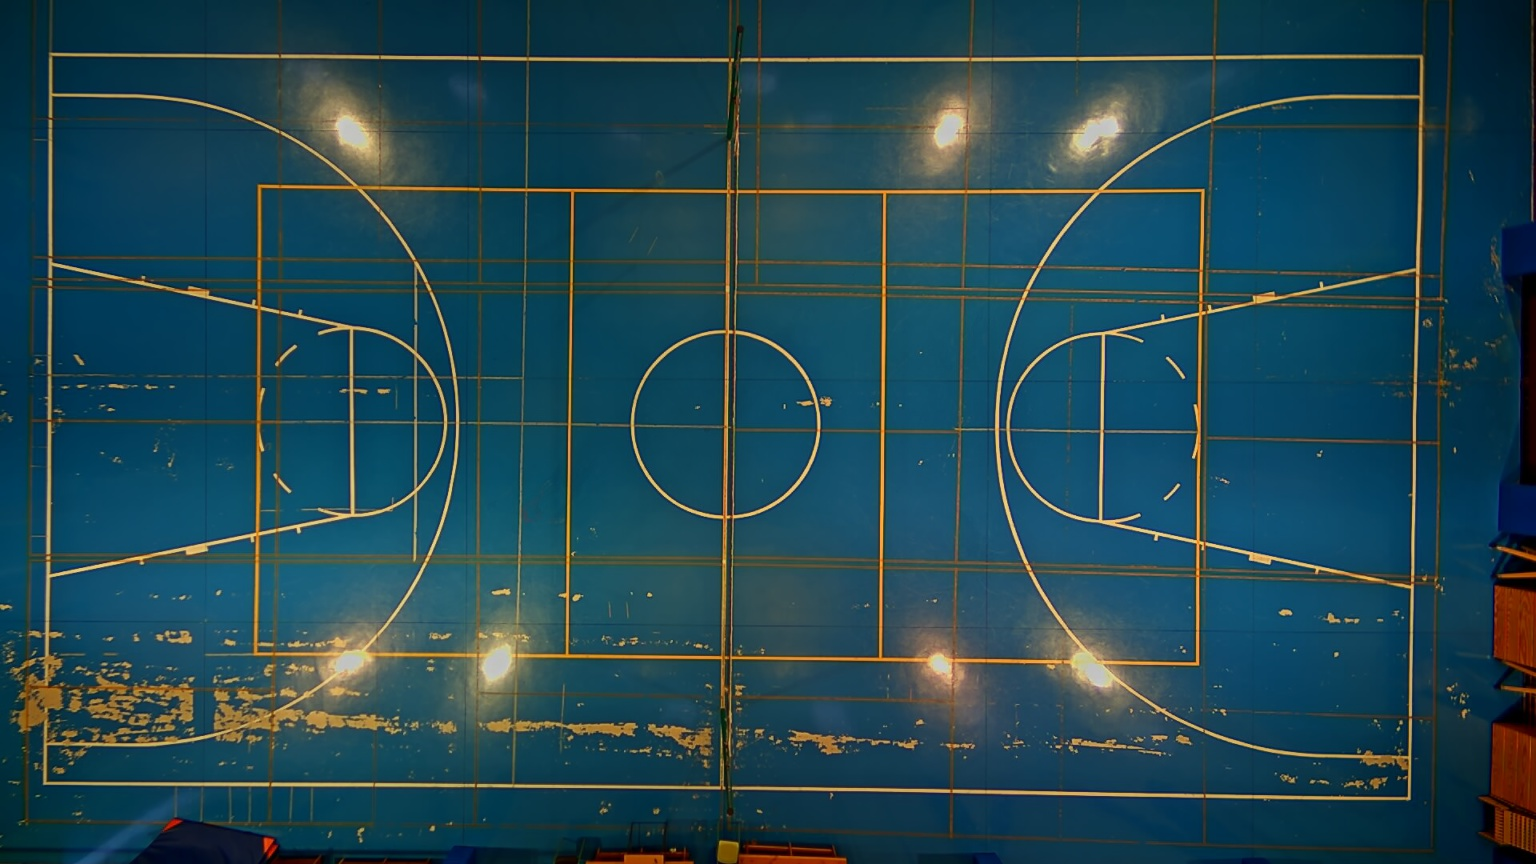
\includegraphics[width=0.6\textwidth]{images/campo}
    \caption{Imagen del campo vacío}
    \label{fig:campo}
\end{figure}

Una vez hecho esto, las posiciones de los jugadores y del balón deberían quedar registrados en un archivo CSV, divididas por jugadas y sets, para su posterior análisis con la intención de extraer estadísticas útiles a nivel técnico. 

Para hacer esta división por jugadas, lo ideal es que el sistema lo haga de forma automática, aunque también podría hacerlo un operario mediante pulsaciones de teclas o mediante el uso de una posible interfaz gráfica.

\subsection{Instalación de cámara en el pabellón}
Un aspecto primordial para este proyecto era la instalación de una cámara que proporcionase las imágenes descritas en la sección anterior. Dicha cámara es un modelo AXIS P1365-E Mk II (figura \ref{fig:camara}), cuyas características, según su ficha técnica, son:

\begin{figure}
    \centering
    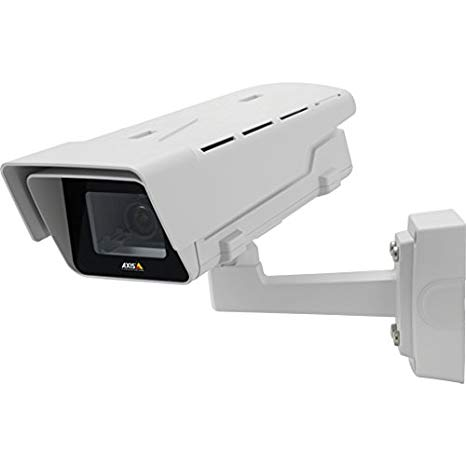
\includegraphics[width=0.5\textwidth]{images/camara}
    \caption{Imagen de la cámara AXIS P1365-E Mk II}
    \label{fig:camara}
\end{figure}

\begin{itemize}
    \item Rango de temperaturas operativas entre -40 ºC y 50 ºC
    \item Resistencia a impactos
    \item Ahorro de ancho de banda mediante tecnología Zipstream
    \item Vídeo a 1080p y hasta 60 fps
\end{itemize}

En nuestro caso, la cámara graba a 1080p y 30fps, con un ancho de banda de 100 Mbps en la transferencia de vídeo. Se conecta mediante power over ethernet. El objetivo de la cámara cuenta con zoom óptico variable, con un \textit{field of view} entre 35-107º en horizontal y 19-67º en vertical. Usando el fov máximo y considerando los dos triángulos rectángulos formados por la vertical de la cámara, el campo y el ángulo de apertura de esta:
\[
    2 \cdot \tan(\frac{107}{2} \cdot \frac{\pi}{180}) = 2.70
\]
el rango de metros visibles en horizontal es de $2.7\cdot altura_{cam}$. El techo del pabellón es de 10,1 metros, con lo cual el rango máximo de la cámara es de 27,27 metros. En vertical, usando la misma fórmula, el rango máximo es de $1.3 \cdot altura_{cam}$, lo que nos da 13,13 metros de rango vertical.

\begin{figure}
\begin{subfigure}{.5\textwidth}
  \centering
  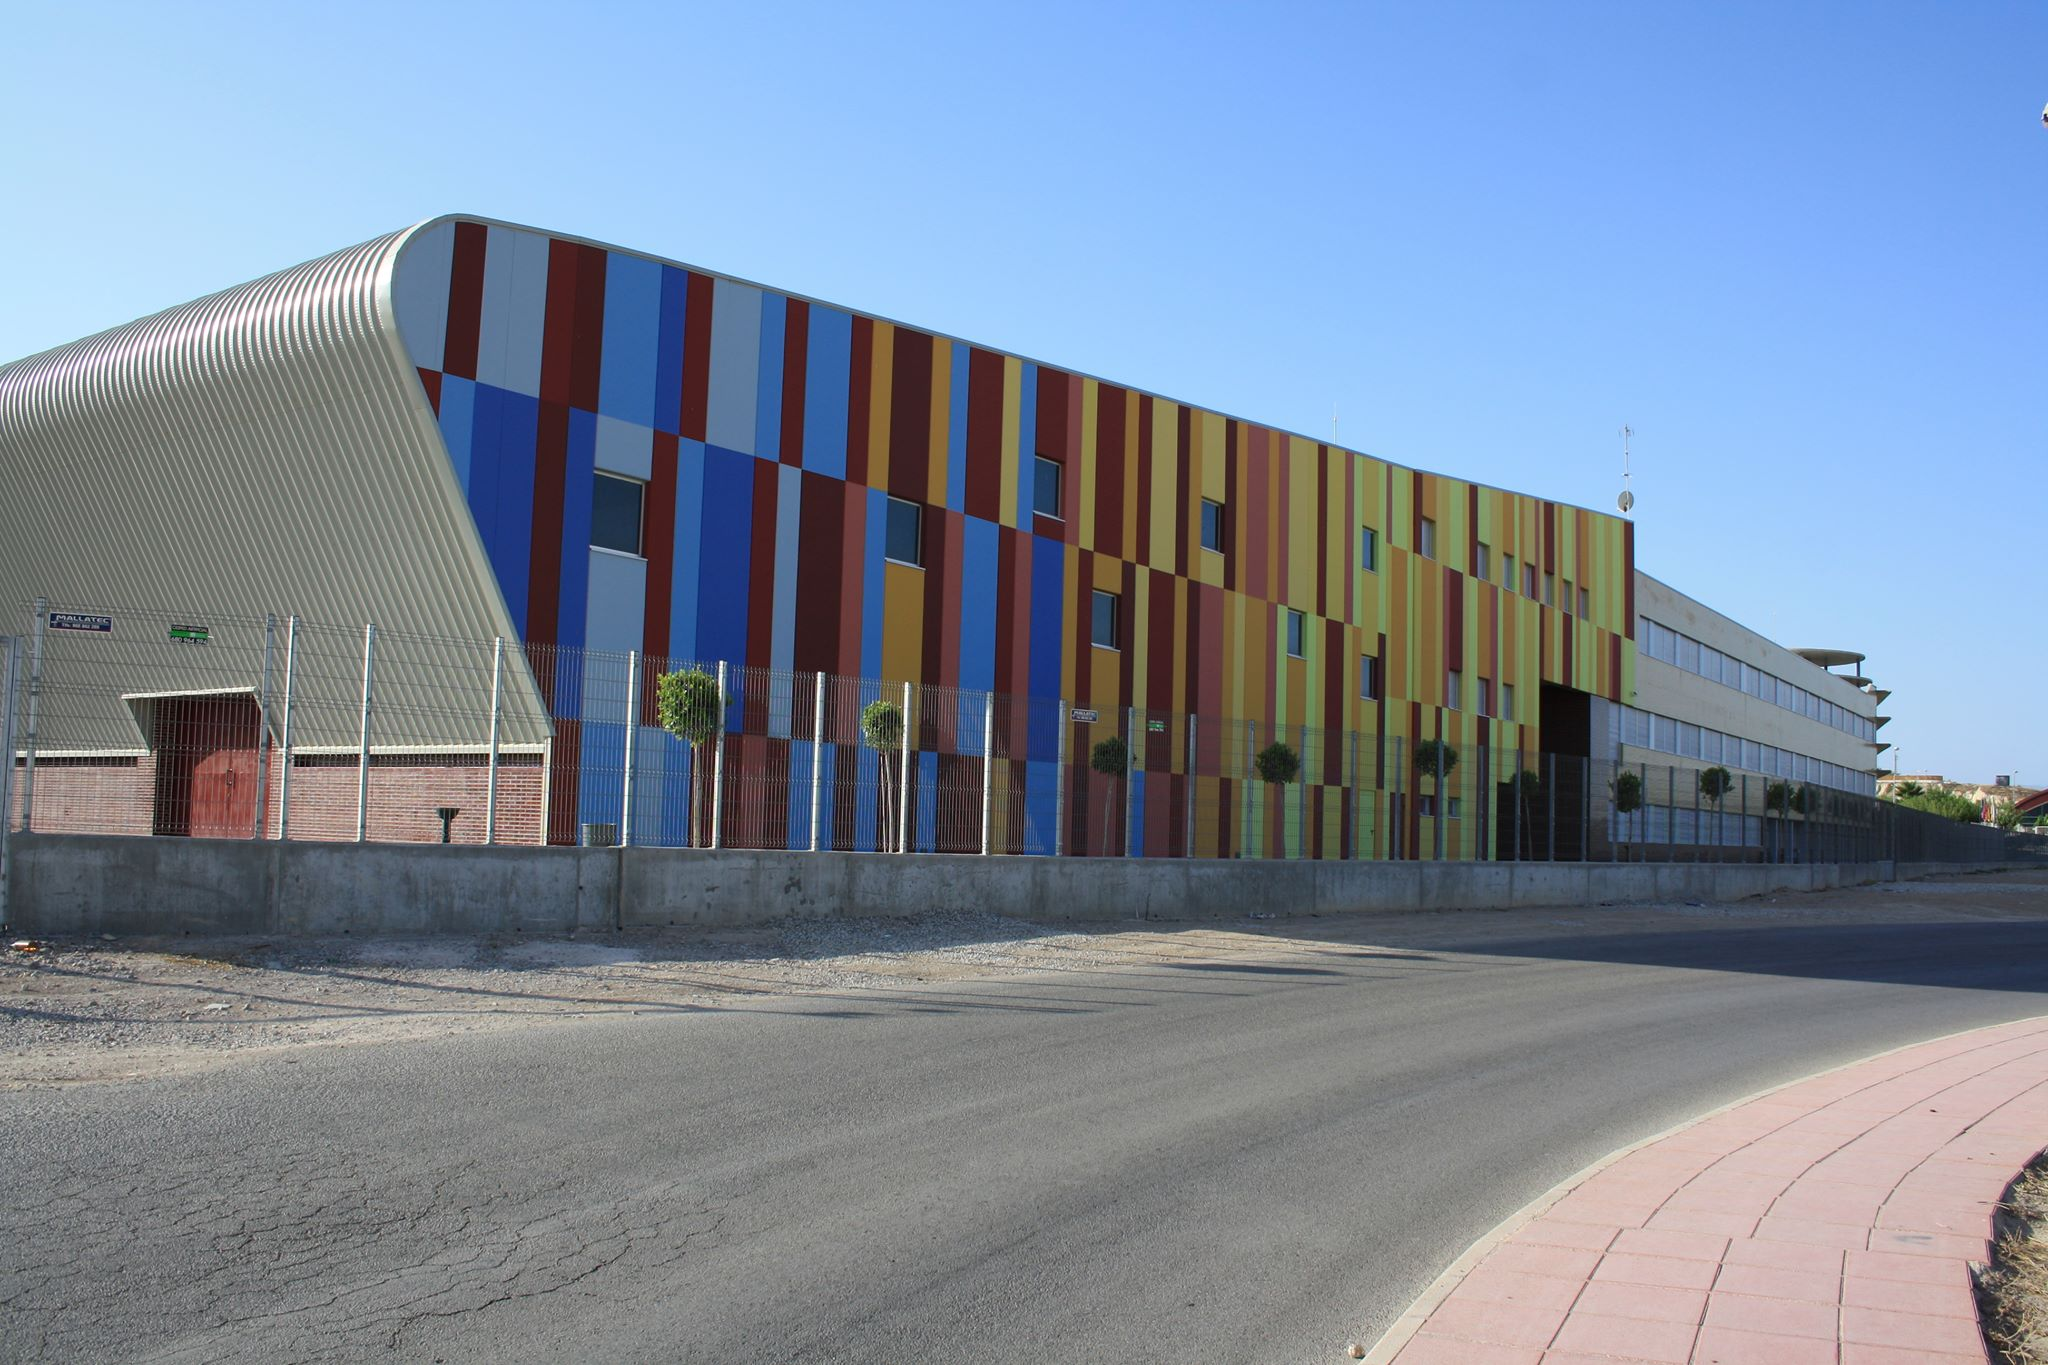
\includegraphics[width=.9\linewidth]{images/EduardoLinares}
  \caption { }
  \label{fig:pabellonFuera}
\end{subfigure}%
\begin{subfigure}{.5\textwidth}
  \centering
  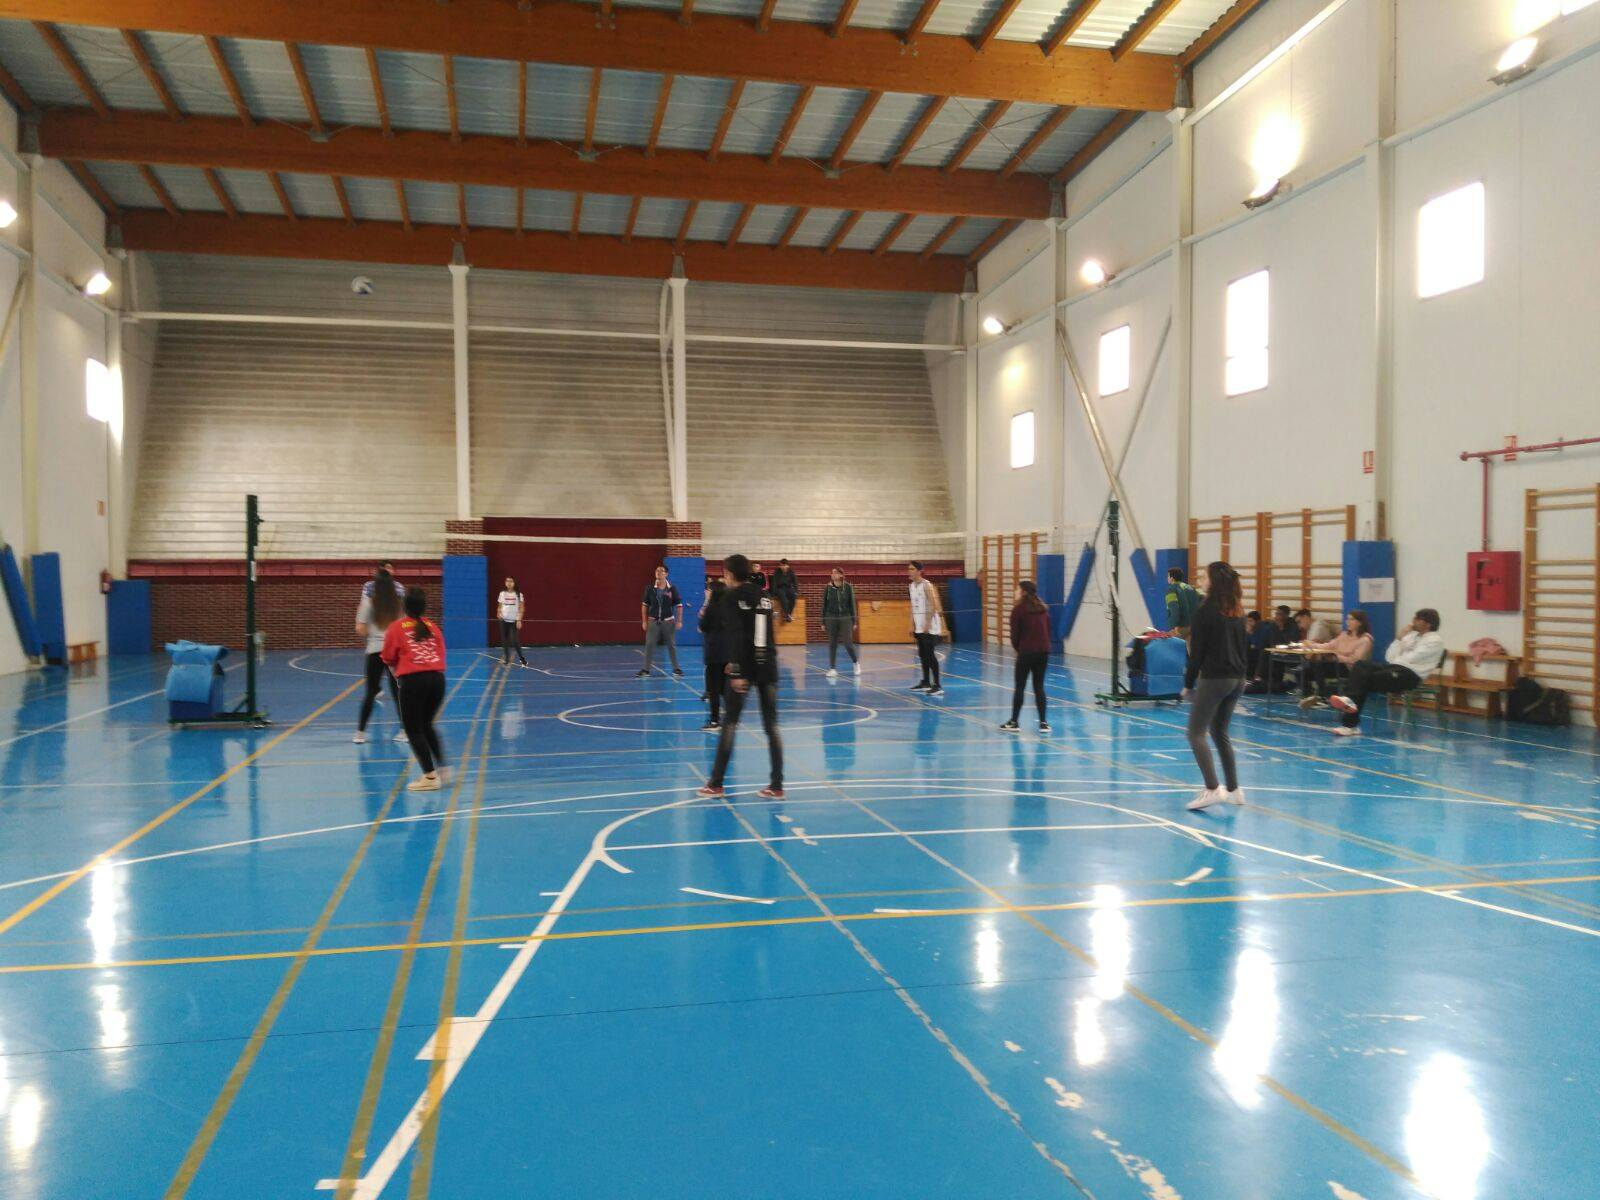
\includegraphics[width=.9\linewidth]{images/EduardoLinaresDentro}
  \caption { }
  \label{fig:pabellonDentro}
\end{subfigure}
\caption{Fotos del exterior (a) y del interior (b) del pabellón Eduardo Linares }
\label{fig:pabellon}
\end{figure}

El pabellón en el que se ha instalado la cámara, previo permiso del Ayuntamiento, es el Eduardo Linares, en Molina de Segura, perteneciente al instituto de Enseñanza Secundaria Eduardo Linares.

\subsection{Herramientas utilizadas y metodología}
Durante la realización de este trabajo se han utilizado una serie de herramientas que pasaré a listar y detallar a continuación.

\subsubsection*{Python}
Python es un lenguaje de programación interpretado, multiparadigma y de tipado dinámico. Nace a finales de los 80, pero alcanzó una mayor popularidad a partir de mediados de los 2000, poco después de la versión 2.0 del lenguaje. En la actualidad, Python es uno de los lenguajes más utilizados en materia de procesado científico y \textit{machine learning}.

La totalidad del desarrollo del software de este trabajo se realizará en este lenguaje. Se ha tomado esta decisión debido a la gran sencillez que aporta, en conjunto con el hecho de que es multiplataforma. Otra gran ventaja del lenguaje es la disponibilidad de librerías como OpenCV, que será la piedra angular del proyecto. 

\subsubsection*{OpenCV}
OpenCV surge en 1999, originalmente desarrollada por Intel, como librería de C++ de visión artificial y \textit{machine learning}. En la actualidad cuenta con versiones para Python, Java, MATLAB entre otros lenguajes. Se encuentra disponible para Linux, Mac y Windows. OpenCV cuenta con implementaciones de más de 2500 algoritmos de visión artificial, que cubren un gran abanico de casos de uso, desde reconocimiento de objetos hasta control de tráfico o seguridad.

Como se ha comentado antes, OpenCV es una parte fundamental de este proyecto, ya que todo lo referente a la visión artificial va a hacer uso de esta librería.

\subsubsection*{Git}
Git es una herramienta de control de versiones originalmente desarrollada por Linus Torvalds para mantener el kernel de Linux. Su desarrollo comienza en abril de 2005 y su primera versión estable se lanzó en diciembre de ese mismo año. En la actualidad se ha convertido en uno de los sistemas de control de versiones más importantes.

El uso de Git (o cualquier VCS) es, en mi opinión, indispensable por pequeña que sea la envergadura del proyecto a desarrollar, debido a la posibilidad de tener siempre disponibles las versiones anteriores del código. Esto hace extremadamente sencillo volver a una versión anterior en caso de necesidad, y proporciona una buena manera de hacer backups incrementales del código. También es muy útil de cara al trabajo en equipo, en nuestro caso, la supervisión de los avances del trabajo por parte del director.

\subsection*{PyQt}
PyQt es una adaptación multiplataforma de la librería gráfica Qt. Esta librería está desarrollada por la compañía inglesa Riverbank Computing. PyQt cuenta con toda la funcionalidad de programación de aplicaciones gráficas disponible en la librería de la que proviene.

PyQt ha facilitado en gran medida la programación de una interfaz gráfica, lo que es interesante de cara a facilitar el uso de la aplicación al usuario medio.